\documentclass[a4paper]{article}
\usepackage[utf8]{inputenc}
\usepackage[T1]{fontenc}
\usepackage{lmodern}
\usepackage{listings}
\usepackage{graphicx}
\usepackage{dirtree}
\usepackage{caption}
\usepackage{subcaption}
\usepackage{float}
\usepackage[english]{babel}
\usepackage[margin=1.1in]{geometry}
\title{HiBoP User Manual}
\author{\textsc{BONTEMPS Benjamin} \\ \textsc{CHATARD Benoît} \\ \textsc{GANNERIE Adrien} \\ \textsc{LANCE Florian} \\ \textsc{SIPP Florian}}
\lstset{
	frame = single,
	basicstyle = \footnotesize\ttfamily
}

\begin{document}
\maketitle
\begin{abstract}
This document is the user manual of the Human Intracranial Brain Observation Player (HiBoP). HiBoP is being developed by the Centre de Recherche en Neurosciences de Lyon (CRNL), with funds from the Human Brain Project (HBP) to visualize large datasets of intracranial electroencephalography (iEEG) and functional MRI data. This document has been written for the 4.0.0 version of HiBoP.
\end{abstract}
\tableofcontents
\section{HiBoP project} \label{data}
\paragraph{} A \textbf{Project} links together anatomical and functional data from a set of patients. If you have an anatomical description of the patients (3D mesh of the brain, MRI and coordinates of the sites of the electrodes) and the respective iEEG data, you can visualize them in 4D (3D space + time). The first thing to do with HiBoP is to create or open a Project. This can be done within HiBoP (section \ref{UI}), but also using a Python API\footnote{This API can be downloaded at https://github.com/hbp-HiBoP/HiBoP-Python-API.} which can automatically generates a project file.
\paragraph{} On your Hard Drive, the Project consists of a .hibop file. This file is in reality a zip archive containing several subfolders (Figure \ref{projectDirectory}). The contents of this archive can be extracted using an unzipping software. Each file is encoded with the json format, and thus can be edited (at your own risks) using any text editor. However this is not recommended, as any coma missing may cause the file to be incorrectly interpreted. You can then zip the folder again and rename the extension from .zip to .hibop.
\begin{figure}[H]
\framebox[\textwidth]{%
\begin{minipage}{0.9\textwidth}
\dirtree{%
	.1 ProjectName.hibop/.
	.2 ProjectName.settings.
	.2 Datasets/.
	.3 DatasetName.dataset.
	.3 ....
	.2 Groups/.
	.3 GroupName.group.
	.3 ....
	.2 Patients/.
	.3 PatientName.patient.
	.3 ....
	.2 Protocols/.
	.3 ProtocolName.prov.
	.3 ....
	.2 Visualizations/.
	.3 VisualizationName.visualization.
	.3 ....
}
\end{minipage}
}
\caption{\label{projectDirectory}Project directory hierarchy}
\end{figure}
\subsection{Settings}
\paragraph{} The .settings file at the root of the project archive describes some project settings. This file contains the name of the project, a default path for the anatomical data of the patients and a default path for the functional data, as well as aliases to shorten paths in other files. It also contains all the tags defined in the project. These tags are used to add more information on the patients or on the sites of the patients.
\subsection{Patients}
\paragraph{} This subfolder contains .patient files, each containing metadata for the patient and its full anatomical description. A 3D mesh can be a single mesh (only one file) or a left-right mesh (one file for the left part and one for the right part of the brain). These files are in GIfTI format (.gii). You can also provide additional files to show MarsAtlas parcels (.gii), or a transformation file (to align the mesh and its respective MRI, .trm). The MRIs must be in the NIfTI-1 format (.nii, .nii.gz, .hdr/.img). These files also contain information about the sites of the patient (position and metadata as tags) and the tags of the patient itself.
\subsection{Groups}
\paragraph{} This subfolder contains .group files, which are simple lists of patients.
\subsection{Protocols}
\paragraph{} This subfolder contains .prov files. The .prov extension stands for \textbf{protocol visualization}. Typically, an iEEG functional data file in HiBoP is a set of time series (one for each channel) with data for each sample from the beginning to the end of the recording session. In addition, information about the events of the experimental paradigm is stored, each event being identified using a code (e.g. an event of code 10 occured at sample 134567).
\paragraph{} The .prov file instructs HiBoP on how to epoch the data based on the events. It consists of blocs which contain a list of subblocs. Each bloc or subbloc will be sorted using first their respective order and then alphabetically using their respective names.
\paragraph{} Each subbloc is centered around a specific event, called \textbf{main event}, for a specific time window (for instance, consider all events with code 10 and extract for each of them a window ranging from 200ms before to 700ms after that event). You can specify secondary events which do not interfere in the epoching. You can also set a baseline window, which is used for the baseline correction (described in more details in Section \ref{preferences}). 
\paragraph{} Each bloc also has a sorting method, which is used to sort the trials obtained from the epoching according to specific conditions (code of the main event, latency of the secondary event...). The syntax used here for a condition is \textit{SUBBLOC\_EVENT\_COMMAND} where SUBBLOC is the name of the sub-bloc, EVENT the name of the event and COMMAND the sorting parameter (which can be LATENCY or CODE). You can specify multiple conditions which are separated by a semi-colon, each of which are interpreted in the order they have been written. The rest of the .prov file is straightforward: you can ask HiBoP to show images (.png or .jpg) at specific time windows, or to associate an image to a bloc. You can also apply treatments on some time windows of the epoched values (e.g. you can compute the absolute value of the values from 100ms to 400ms after the main event).
\paragraph{} \textbf{Important note:} You need to make a whole protocol with blocs and subblocs only if you want to visualize iEEG or CCEP data. In the case of fMRI, you only need to create an empty protocol (which is still required to organize the data).
\subsection{Datasets}
\paragraph{} This subfolder contains .dataset files, which summarize and link together anatomical and functional data for a given cognitive task. A dataset is a list of data information (datainfo), each of them connecting one patient (and its anatomical data) to functional data for a single experiment.
\paragraph{} A datainfo can be of type iEEG, CCEP, fMRI, MEGc or MEGv. In the case of iEEG, you can specify a normalization method (see Section \ref{preferences} for detailed information about normalization). In the case of CCEP, you have to specify the channel that has been stimulated. MEGc corresponds to MEG data represented as time series (similar to iEEG) and MEGv corresponds to MEG data represented in voxels (similar to fMRI). Each datainfo contains a data container which handles the data files.
\paragraph{} A data container can be of type ELAN\footnote{\label{ELAN}ELAN format – ELAN is freely available at http://elan.lyon.inserm.fr}, Micromed, BrainVision, EDF, NIFTI-1 or FIF. Each datainfo type can handle some of these data types:
\begin{itemize}
\item \textbf{iEEG}: ELAN, Micromed, BrainVision, EDF
\item \textbf{CCEP}: ELAN, Micromed, BrainVision, EDF
\item \textbf{fMRI}: NIFTI-1
\item \textbf{MEGc}: BrainVision, EDF, FIF
\item \textbf{MEGv}: NIFTI-1
\end{itemize}
\subsection{Visualizations}
\paragraph{} This subfolder contains .visualization files, which describe the contents of a visualization: it is composed of patients and columns. Each column allow one to visualize either the anatomy of the chosen patients or iEEG/CCEP/fMRI/MEG\footnote{\label{MEG}In the case of a MEG column, MEGc and MEGv data will be used together if they both have the same data name set in the MEG column.} data. The file also stores the configuration of the visualization (most of the parameters modified within the visualization can be saved as the configuration of the visualization).
\section{HiBoP description}\label{UI}
\paragraph{} This section will describe in details how to use HiBoP to create a HiBoP project and how to visualize the data. The first thing to do is to open HiBoP (if you need them, instructions are in the README.md file located next to the executable). If you have any doubt about what an interface element does, you can hover it for a second and a tooltip will appear telling you what it does.
\subsection{User Preferences}\label{preferences}
\paragraph{} A lot of global parameters shared through all projects can be set using the preferences menu (Figure \ref{preferencesUI}). The menu contains 3 tabs each containing submenus. These parameters are stored in the persistent data folder of HiBoP\footnote{See https://docs.unity3d.com/ScriptReference/Application-persistentDataPath.html for more information (with companyname being CRNL and productname being HiBoP).}.
\begin{figure}[H]
\begin{center}
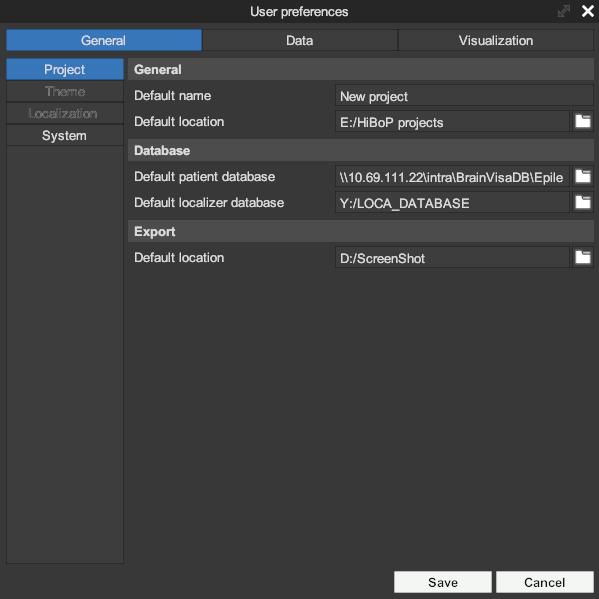
\includegraphics[scale=0.5]{Preferences.png}
\end{center}
\caption{\label{preferencesUI}User Preferences}
\end{figure}
\begin{itemize}
\item \textbf{General}
\begin{itemize}
\item \textbf{Project}
\begin{itemize}
\item \textbf{General}
\begin{itemize}
\item \textbf{Default name}: Default name for a new project
\item \textbf{Default location}: Default path to search for projects
\end{itemize}
\item \textbf{Database}
\begin{itemize}
\item \textbf{Default patient database}: Default path to the patient database
\item \textbf{Default localizer database}: Default path to functional data
\end{itemize}
\item \textbf{Export}
\begin{itemize}
\item \textbf{Default location}: Default path to save screenshots
\end{itemize}
\end{itemize}
\item \textbf{System}
\begin{itemize}
\item \textbf{Performance}
\begin{itemize}
\item \textbf{Enable multithreading}: Enable multithreading for calculation (e.g. EEG signal on the brain mesh)
\item \textbf{Memory cache limit}: Maximum amount of memory taken by HiBoP
\item \textbf{Target framerate}: Maximum amount of frames displayed each second
\item \textbf{Sleep mode}: Time before HiBoP enters sleep mode, reducing used computer resources
\end{itemize}
\end{itemize}
\end{itemize}
\item \textbf{Data}
\begin{itemize}
\item \textbf{EEG}
\begin{itemize}
\item \textbf{Processing}
\begin{itemize}
\item \textbf{Averaging method}: Method to average the data (mean or median)
\item \textbf{Normalizing method}: The following formula is applied to each value $v$ $$v = \frac{v - \mu_{b}}{\sigma_{b}}$$ where $b$ is an array of the baseline values depending on this parameter, $\mu_b$ is their mean and $\sigma_b$ is their standard deviation
\end{itemize}
\item \textbf{Correlations}
\begin{itemize}
\item \textbf{Alpha threshold}: Alpha value to be compared to the p-values resulting from the Wilcoxon test when computing correlations between channels (see Appendix \ref{correlations} for more information)
\item \textbf{Use Bonferroni correction}: If true, the alpha value set above will be divided by the number of Wilcoxon tests performed, that is $\frac{N \times (N - 1)}{2}$ for $N$ channels
\end{itemize}
\end{itemize}
\item \textbf{Protocol}
\begin{itemize}
\item \textbf{Time window}
\begin{itemize}
\item \textbf{Maximum range}: The maximum range for the time window of a subbloc of a protocol
\item \textbf{Step}: The step between two positions of the range slider when editing the time window of a protocol
\end{itemize}
\end{itemize}
\begin{itemize}
\item \textbf{Processing}
\begin{itemize}
\item \textbf{Position averaging method}: Method to average the position of the secondary events (mean or median)
\end{itemize}
\end{itemize}
\item \textbf{Anatomy}
\begin{itemize}
\item \textbf{Performances}
\begin{itemize}
\item \textbf{Enable mesh preloading}: Preload every meshes at the start of a visualization
\item \textbf{Enable MRI preloading}: Preload every MRIs at the start of a visualization
\item \textbf{Enable implantation preloading}: Preload every implantations at the start of a visualization
\item \textbf{Preload all patient data in multi-patient visualizations}: Each time you open a multi-patient visualization, the anatomical data of all the patients will be loaded in order to make the transitions between multi-patient and single-patient visualizations smoother. Be careful, this setting can take a lot of memory.
\end{itemize}
\item \textbf{Processing}
\begin{itemize}
\item \textbf{Enable site name correction}: Change the name of a certain patern of site names when importing sites from a file (for instance "xp4" becomes "X'4")
\end{itemize}
\end{itemize}
\end{itemize}
\item \textbf{Atlases}
\begin{itemize}
\item \textbf{Preload X atlas on startup}: If checked, the corresponding atlas will be loaded at the start of HiBoP. The amount of memory taken is written in brackets. You can also manually load each atlas, and visit the website of the atlas.
\end{itemize}
\item \textbf{Visualization}
\begin{itemize}
\item \textbf{3D}
\begin{itemize}
\item \textbf{EEG}
\begin{itemize}
\item \textbf{Enable automatic EEG update}: Triggers the update of the brain activity on the brain each time a parameter is changed in the visualization
\item \textbf{Site influence by distance}: Controls how a site influence its environment (constant amplitude, linear decrease or quadratic decrease)
\end{itemize}
\item \textbf{Display}
\begin{itemize}
\item \textbf{Visualizations layout}: Layout to use when multiple visualizations are open at the same time
\end{itemize}
\item \textbf{Single/Multi patient visualization}
\begin{itemize}
\item \textbf{Default selected MRI}: Select the MRI corresponding to this name when loading a new visualization, or the first in the list if the name does not match any
\item \textbf{Default selected mesh}: Select the mesh corresponding to this name when loading a new visualization, or the first in the list if the name does not match any
\item \textbf{Default selected implantation}: Select the implantation corresponding to this name when loading a new visualization, or the first in the list if the name does not match any
\end{itemize}
\end{itemize}
\item \textbf{Trial Matrix}
\begin{itemize}
\item \textbf{General}
\begin{itemize}
\item \textbf{Show whole protocol}: Display the matrices of all blocs of a protocol even if no column is set with some blocs of the protocol
\item \textbf{Enable trials synchronization}: Synchronize selected trials when comparing matrices of two sites
\end{itemize}
\item \textbf{Smoothing}
\begin{itemize}
\item \textbf{Enable trial smoothing}: Smoothes the trials of a matrix
\item \textbf{Number of intermediate values}: Number of values to be added between two real values during smoothing process
\end{itemize}
\item \textbf{Format}
\begin{itemize}
\item \textbf{Bloc format}: Changes how a bloc of the matrix is rendered (trials height in pixels, trial ratio or bloc ratio)
\end{itemize}
\end{itemize}
\item \textbf{Graph}
\begin{itemize}
\item \textbf{General}
\begin{itemize}
\item \textbf{Show curves of minimized columns}: Display all curves even if the corresponding column is minimized
\end{itemize}
\item \textbf{Colors}: Set up the colors of the graphs
\end{itemize}
\item \textbf{Cut}
\begin{itemize}
\item \textbf{Display}
\begin{itemize}
\item \textbf{Enable cut lines}: Display other cuts by lines on cut textures
\end{itemize}
\end{itemize}
\end{itemize}
\end{itemize}
\subsection{Project management}
\subsubsection{Creating, opening and saving a project}
\paragraph{} When creating a new project, you have to specify the name of your new project, the location where it will be saved, the location of the anatomical database and the location of the functional database (Figure \ref{newProjectUI}). The two last fields are optional but will create two aliases to shorten the paths to the data files.
\begin{figure}[H]
\begin{center}
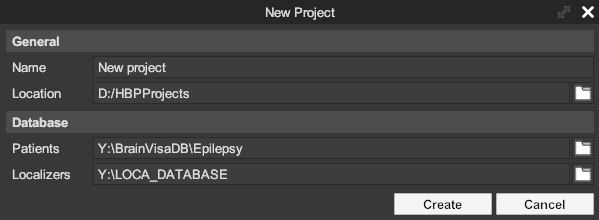
\includegraphics[scale=0.5]{NewProject.png}
\end{center}
\caption{\label{newProjectUI}Create a new project}
\end{figure}
\paragraph{} In order to open a previously created project (Figure \ref{openProjectUI}), you have to tell where your projects are located. Once these are loaded, you can either double click on the project you want to open or select the project and then click on Open. You can also sort projects using specific parameters.
\begin{figure}[H]
\begin{center}
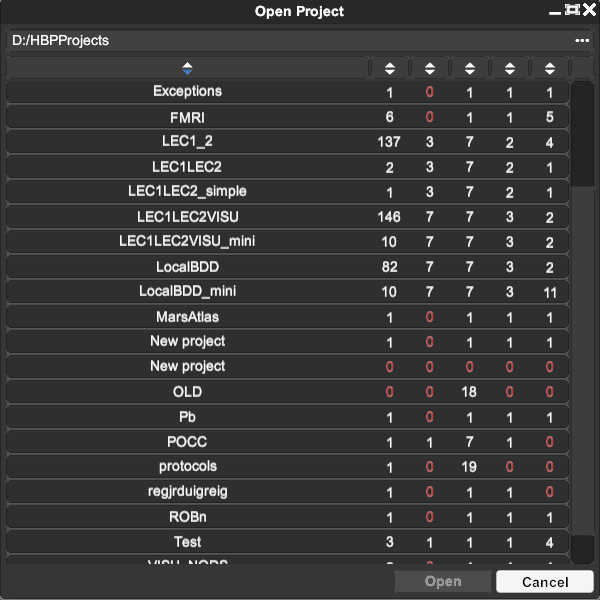
\includegraphics[scale=0.5]{OpenProject.png}
\end{center}
\caption{\label{openProjectUI}Open a project}
\end{figure}
\paragraph{} If you want to save a project to a different location or with a different name than when it was open, you can use the "Save as" menu (Figure \ref{saveProjectUI}).
\begin{figure}[H]
\begin{center}
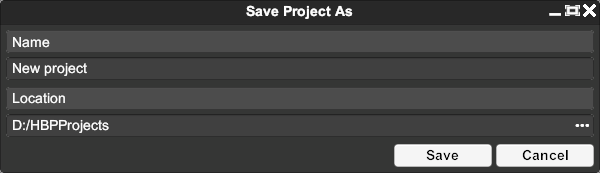
\includegraphics[scale=0.5]{SaveAs.png}
\end{center}
\caption{\label{saveProjectUI}Save a project as}
\end{figure}
\paragraph{} All of these menus are located in the File menu at the top of the screen.
\subsubsection{Patients management}
\paragraph{} To add patients to the opened project, you have to use the patients manager (Figure \ref{patientGestionUI}). This window is composed of a list of all patients in the project, a button to add new patients and a button to remove the selected patients from the list. For each patient, numbers indicate the status of their respective anatomical data (Meshes, MRIs, Sites and Tags). To add or remove patients, follow the instructions described in appendix \ref{addobjects}.
\begin{figure}[H]
\begin{center}
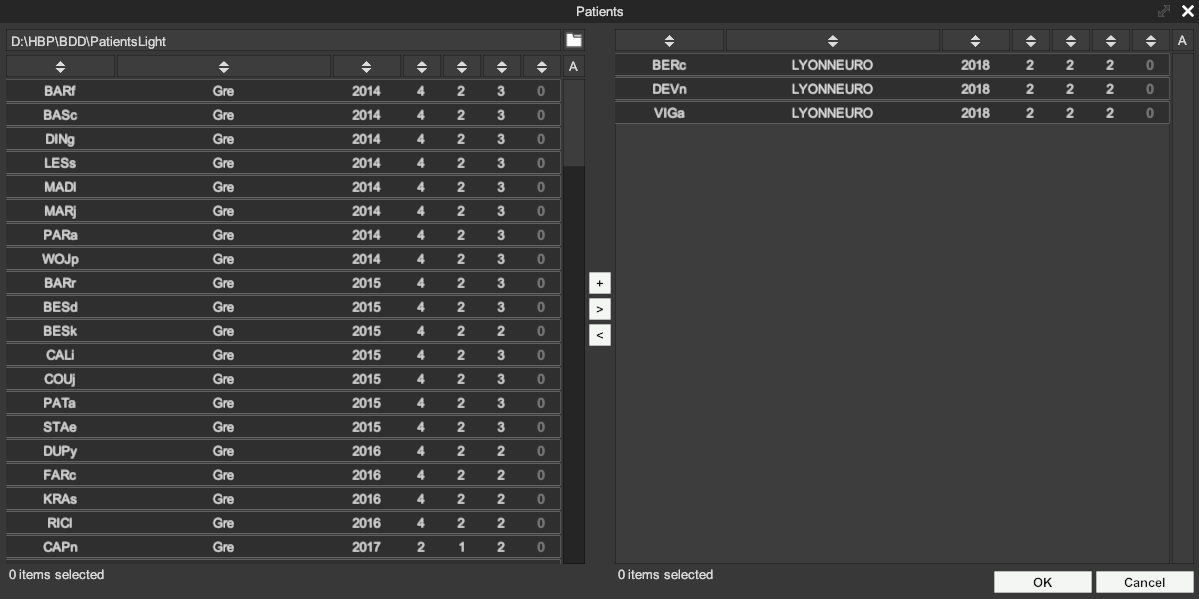
\includegraphics[scale=0.5]{PatientGestion.png}
\end{center}
\caption{\label{patientGestionUI}Patients manager}
\end{figure}
\paragraph{} To edit any loaded patient, you can double click\footnote{The process of double clicking an item to edit it is common to most windows of HiBoP} on it. This will open the patient modifier window (Figure \ref{patientModifierUI}) which will allow you to edit anything concerning the metadata or the anatomical data of this patient. You can navigate between anatomical data types using the tabs in the middle of the window.
\begin{figure}[H]
\begin{center}
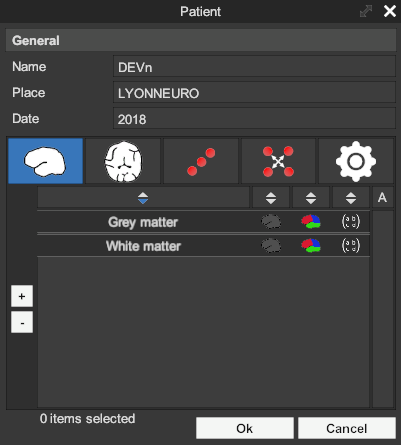
\includegraphics[scale=0.5]{PatientModifier.png}
\end{center}
\caption{\label{patientModifierUI}Patient modifier}
\end{figure}
\paragraph{} As stated in section \ref{data}, you can also create groups of patients to add them more easily to the visualizations. This is done through the groups manager window (Figure \ref{groupGestionUI}). Adding and removing patients from a group is very similar to the patients manager window (Figure \ref{groupModifierUI}).
\begin{figure}[H]
\begin{center}
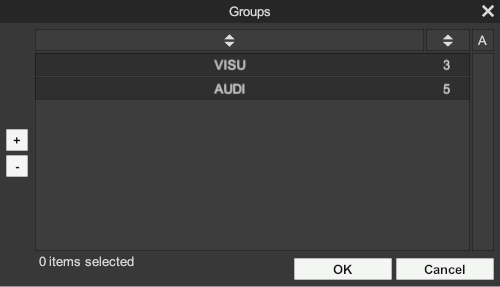
\includegraphics[scale=0.5]{GroupGestion.png}
\end{center}
\caption{\label{groupGestionUI}Groups manager}
\end{figure}
\begin{figure}[H]
\begin{center}
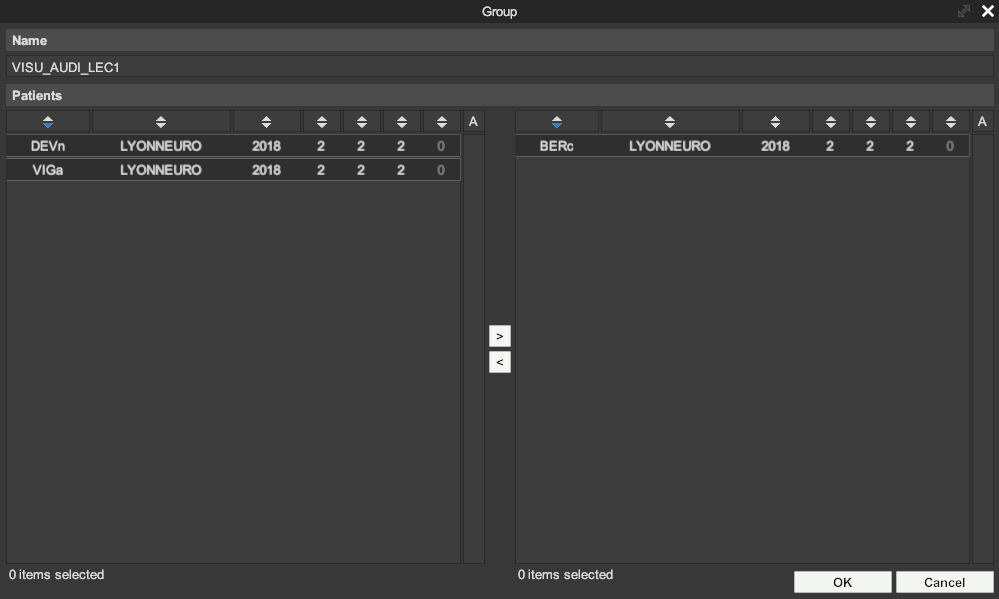
\includegraphics[scale=0.5]{GroupModifier.png}
\end{center}
\caption{\label{groupModifierUI}Group modifier}
\end{figure}
\subsubsection{Functional data management}
\paragraph{} The first thing to do concerning functional data management is to create a protocol. This protocol will be used to epoch the iEEG data, but is also mandatory for other types of data such as fMRI (because a dataset requires a protocol). In the case of data that do not need to be epoched, you do not need to create any bloc for the protocol. You can create a protocol using the protocol manager window (Figure \ref{protocolGestionUI}).
\begin{figure}[H]
\begin{center}
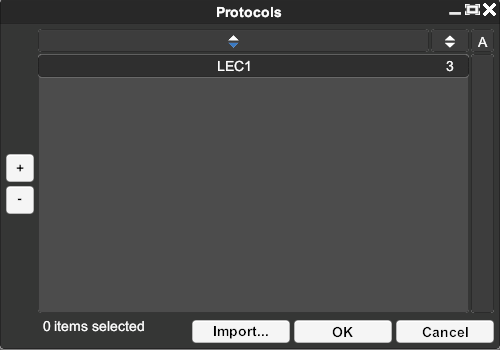
\includegraphics[scale=0.5]{ProtocolGestion.png}
\end{center}
\caption{\label{protocolGestionUI}Protocols manager}
\end{figure}
\paragraph{} Editing a protocol consists of defining the blocs for this protocol. This is done with the protocol modifier window (Figure \ref{protocolModifierUI}).
\begin{figure}[H]
\begin{center}
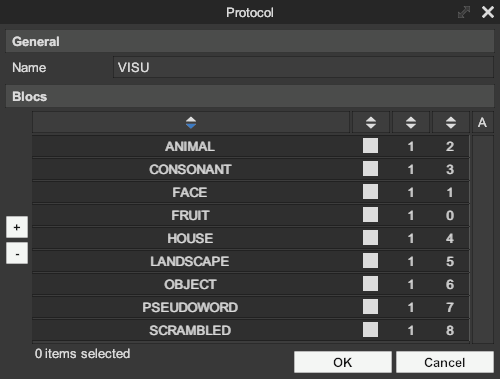
\includegraphics[scale=0.5]{ProtocolModifier.png}
\end{center}
\caption{\label{protocolModifierUI}Protocol modifier}
\end{figure}
\paragraph{} A bloc can be edited with the bloc modifier window (Figure \ref{blocModifierUI}). There you can specify the name, the sorting method, and define the subblocs using the subbloc modifier window (Figure \ref{subBlocModifierUI}). There, you can edit the name, the order, the type (main or secondary), the window, the baseline window, the events, the iconic scenario and the treatments of the subbloc.
\begin{figure}[H]
\begin{center}
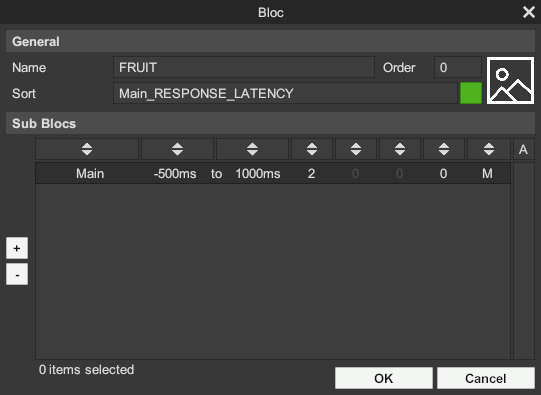
\includegraphics[scale=0.5]{BlocModifier.png}
\end{center}
\caption{\label{blocModifierUI}Bloc modifier}
\end{figure}
\begin{figure}[H]
\begin{center}
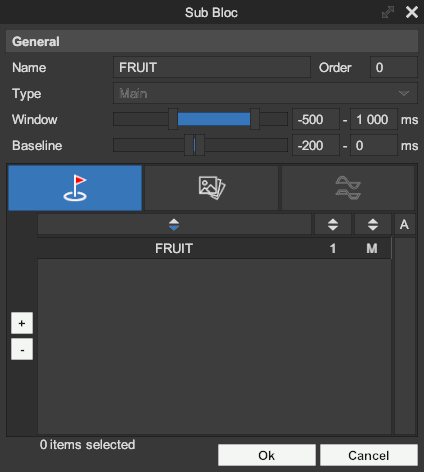
\includegraphics[scale=0.5]{SubBlocModifier.png}
\end{center}
\caption{\label{subBlocModifierUI}SubBloc modifier}
\end{figure}
\paragraph{} When your protocols are correctly defined, you are ready to create your datasets. This will be done using the datasets manager window (Figure \ref{datasetGestionUI}).
\begin{figure}[H]
\begin{center}
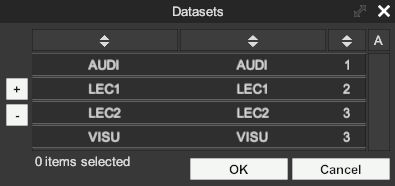
\includegraphics[scale=0.5]{DatasetGestion.png}
\end{center}
\caption{\label{datasetGestionUI}Datasets manager}
\end{figure}
\paragraph{} For a given dataset, you need to give it a name and assign a protocol. All the data included in this dataset will be epoched regarding the chosen protocol. With the dataset modifier window (Figure \ref{datasetModifierUI}), you can add and edit data information. Each data information has a little colored box which indicates the status of the data information : red means it is unsuable, whereas green means you can visualize it. You can hover this box to have more information about the data information status.
\begin{figure}[H]
\begin{center}
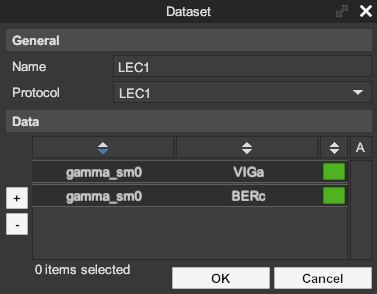
\includegraphics[scale=0.5]{DatasetModifier.png}
\end{center}
\caption{\label{datasetModifierUI}Dataset modifier}
\end{figure}
\paragraph{} A data information has a name and is linked to a patient. A data information can be either an iEEG, CCEP, fMRI or MEG data information. In the case of an iEEG data information, you can specify the normalization method for this specific data (this overwrites the global parameter for normalization unless "Auto" is selected), and there can only be one data information for each [name, patient]. In the case of a CCEP data information, you have to specify the stimulated site for this data, and there can only be one data information for each [name, patient, stimulated site]. In the case of a fMRI data information, there can only be one data information for each [name, patient]. In the case of a MEG data information, there can only be one data information for each [name, patient] for each MEG data category (MEGc and MEGv). If a MEGc and a MEGv data information share the same name and the same patient, they will both be loaded in the corresponding MEG column.
\paragraph{} Data information are identified by their names, so if you want to visualize data of several patients in the same column, you have to give them the same name. As for the data you can choose the data format and fill all the required fields.
\begin{figure}[H]
\begin{center}
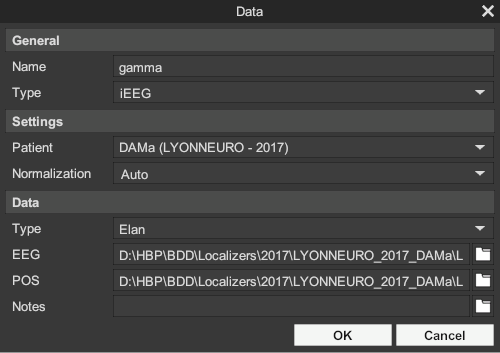
\includegraphics[scale=0.5]{DataInfoModifier.png}
\end{center}
\caption{\label{dataInfoModifierUI}Data information modifier}
\end{figure}
\subsubsection{Visualizations management}
\paragraph{} When everything is set up, you can create visualizations. This is done using the visualization manager window (Figure \ref{visuGestionUI}).
\begin{figure}[H]
\begin{center}
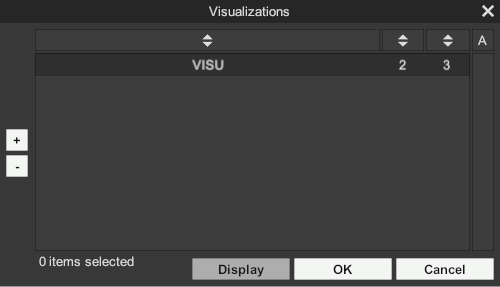
\includegraphics[scale=0.5]{VisualizationGestion.png}
\end{center}
\caption{\label{visuGestionUI}Visualizations manager}
\end{figure}
\paragraph{} A visualization has a name, patients and columns. To edit all of this information, you can use the visualization modifier window (Figure \ref{visuModifierUI}). To add a column, click on the "+" button under the "Columns" panel. You can then edit the column by setting the name, the type (Anatomy, iEEG, CCEP, fMRI or MEG), the protocol, the bloc, the dataset and the data name to be used in this column. Do not forget that if multiple patients are added to the visualization, they must have at least one data information with the same name. If this condition is not matched, there will be a warning you can hover to see which patient is problematic.
\begin{figure}[H]
\begin{center}
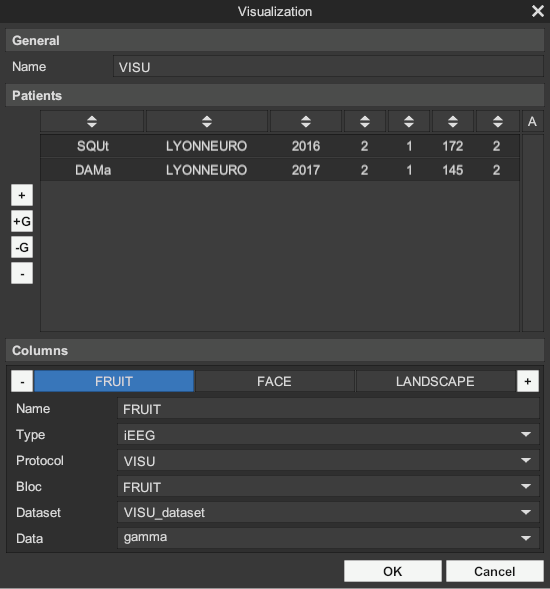
\includegraphics[scale=0.4]{VisualizationModifier.png}
\end{center}
\caption{\label{visuModifierUI}Visualization modifier}
\end{figure}
\paragraph{} Once your visualizations are ready to be displayed, you can select them and click the "Display" button.
\subsection{3D Visualization}
\paragraph{}
\begin{figure}[H]
\begin{center}
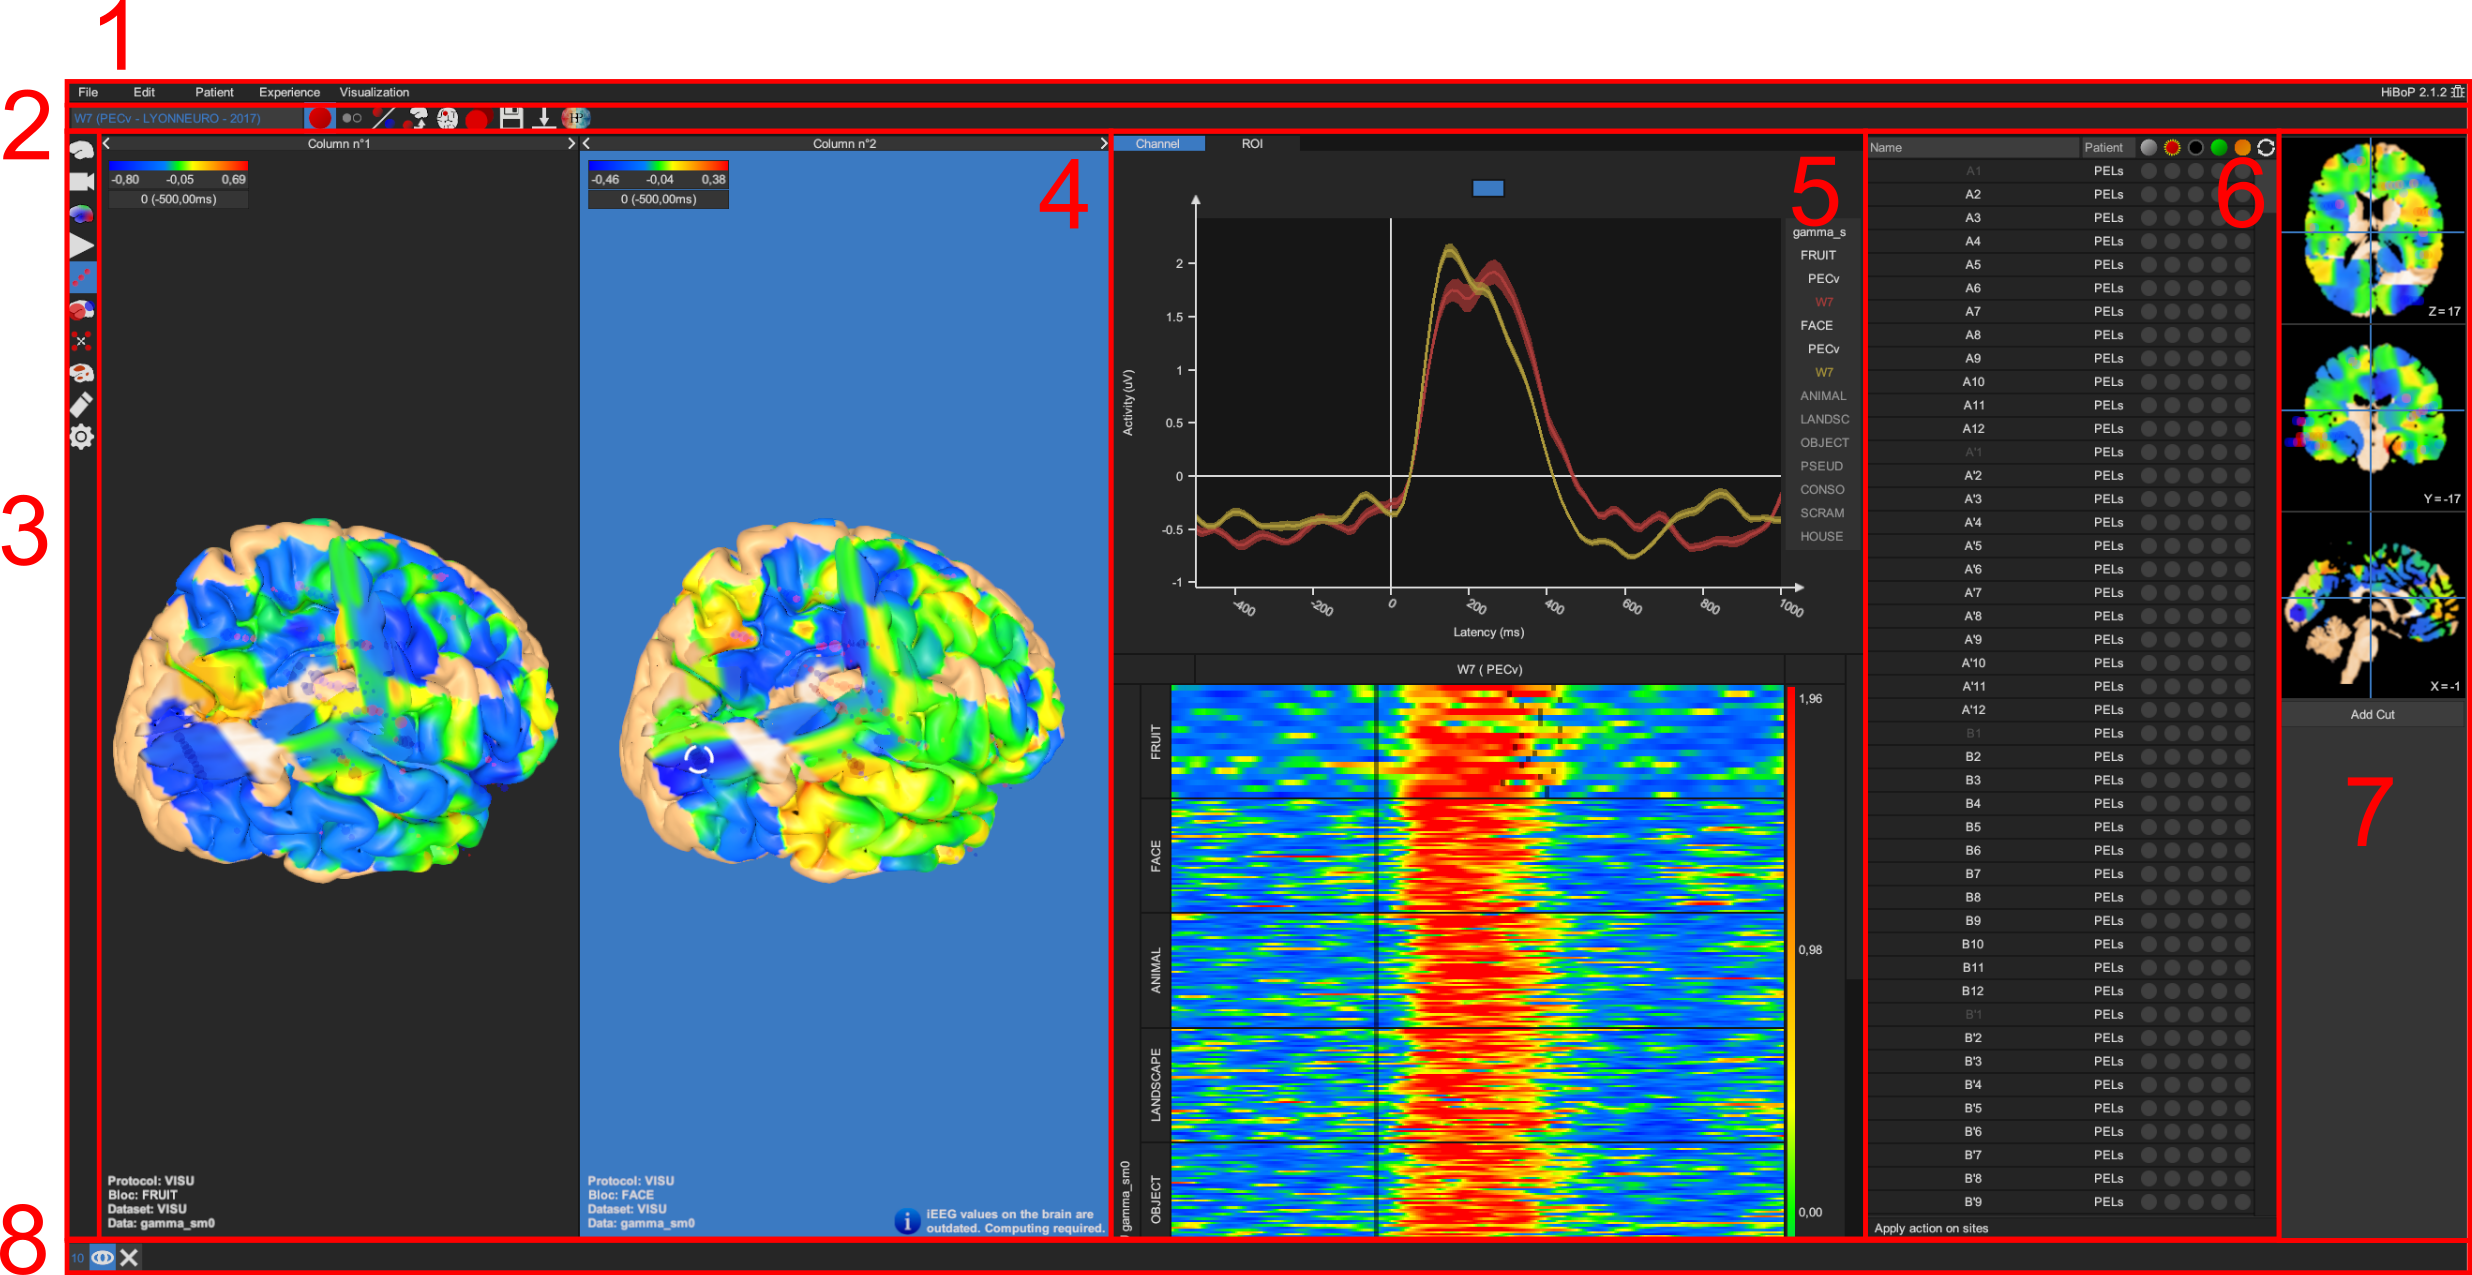
\includegraphics[scale=0.22]{GlobalUI.png}
\end{center}
\caption{\label{globalUI}HiBoP user interface}
\end{figure}
\paragraph{} The main user interface of HiBoP can be decomposed as follow (Figure \ref{globalUI}) :
\begin{itemize}
\item \textbf{1} - Main menu (data management, see section \ref{UI} for more information)
\item \textbf{2} - Toolbar (used to do actions on the 3D scene, more information in later sections)
\item \textbf{3} - Toolbar selector (to select which toolbar you want to use)
\item \textbf{4} - 3D visualization (main visualization window)
\item \textbf{5} - Graphs and trial matrices (precise information of iEEG data, see section \ref{graphs})
\item \textbf{6} - Sites list (manage site states, see section \ref{sitesList})
\item \textbf{7} - Cut panel (manage cuts, see section \ref{cuts})
\item \textbf{8} - Opened visualizations (used to minimize or close opened visualizations)
\end{itemize}
\paragraph{} Elements in parts 4, 5 and 6 can be resized using the black handlers betweens them. Columns of the 3D vizualisations can be moved by drag and dropping their labels at the top of the column. You can interact with the scene in many ways :
\begin{itemize}
\item Left click on a view to select the corresponding view / column / scene or left click on a site / on a ROI to select it.
\item Right click and drag to rotate the brain surface
\item Middle click and drag to translate the brain surface
\item Use the scroll wheel to control the zoom
\item Drag and drop the name of a column to swap it with another column or to insert it between two columns
\end{itemize}
\paragraph{} The left panel allows you to change between toolbars. Each toolbar has its own functions, which will be explained in more details in later sections.
\newline
\begin{minipage}{0.3\textwidth}
\begin{figure}[H]
\begin{center}

\includegraphics[scale=0.89]{ToolbarSelector.png}
\end{center}
\end{figure}
\end{minipage}
\begin{minipage}{0.5\textwidth}
\begin{itemize}
\item Scene settings
\item Display settings
\item Activity settings
\item Timeline
\item Sites
\item Regions of Interest
\item Atlas
\item Triangle eraser
\item Configuration
\end{itemize}
\end{minipage}
\subsubsection{Cuts}\label{cuts}
\paragraph{} Before getting into the toolbars, let's talk about cuts. Indeed, HiBoP allows you to cut the 3D mesh (using the MRI to fill the cut plane) with the right panel. To add a cut, click on the "Add cut" button. You can change parameters on the cut after clicking on it to open the parameters panel (Figure \ref{cut}). You can change its orientation (Axial, Coronal, Sagital or Custom), you can flip it (Axial, Coronal and Sagital) or set up a custom normal (Custom), you can change the position of the cut using the slider or the "+" and "-" buttons for more precision. To delete a cut, open the parameters panel and click on the little cross on the top-right of the cut.
\begin{figure}[H]
\begin{center}
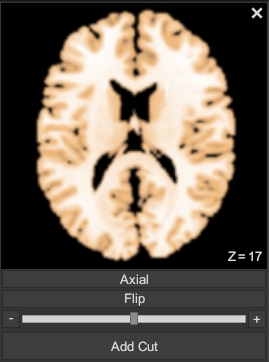
\includegraphics[scale=0.5]{Cut.png}
\end{center}
\caption{\label{cut}Cut parameters panel}
\end{figure}
\subsubsection{Sites list}\label{sitesList}
\paragraph{} A list of all the sites of the scene is available in the corresponding panel (Figure \ref{sitesListPanel}). This list displays all sites of the visualization and their attributes. You can highlight or blacklist a site, change its color and set labels.
\begin{figure}[H]
\begin{center}
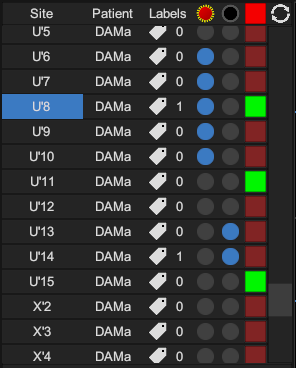
\includegraphics[scale=0.5]{SitesList.png}
\end{center}
\caption{\label{sitesListPanel}Sites list panel}
\end{figure}
\paragraph{} This panel also contains a submenu called "Filter sites" which allows you to filter the sites using various criteria. Only the filtered sites will then appear in the list and on the 3D scene. There are two ways of filtering the sites:
\begin{itemize}
\item You can filter sites using specific conditions concerning their current states, their location, information about them or the EEG signal of the associated channel (Figure \ref{basicStates}).
\item The "Advanced" way can be accessed through the Advanced tab of the aforementioned submenu. While the Basic tab can only filter sites with a global AND between all conditions (which means that all conditions must be fulfilled for a site in order to apply the states), the Advanced tab can be used to create more complex conditions. You can click on the "?" icon to have a detailed description on how it works, alongside examples.
\end{itemize}
\paragraph{} Once you have filtered the sites you can apply an action on them using the "Apply action on filtered sites". There are multiple actions available:
\begin{itemize}
\item You can highlight, unhighlight, blacklist, unblacklist, change the color and add labels to the filtered sites. This allows you to set the states of multiple sites at once, which is conveniant compared to setting the states one by one (Figure \ref{sitesAction}).
\item You can export a list of the filtered sites to a csv file. This file contains the name, the patient name, place and date, the coordinates of the site and the coordinate system used, the data files of the corresponding channel and every tags of the site.
\item You can display the mean curve of all the filtered sites in the Graph panel (more information in section \ref{graphs})
\end{itemize}
\begin{figure}[H]
\begin{center}
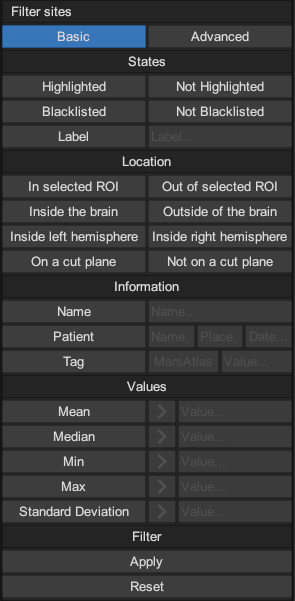
\includegraphics[scale=0.5]{BasicStates.png}
\end{center}
\caption{\label{basicStates}"Filter sites" submenu}
\end{figure}
\begin{figure}[H]
\begin{center}
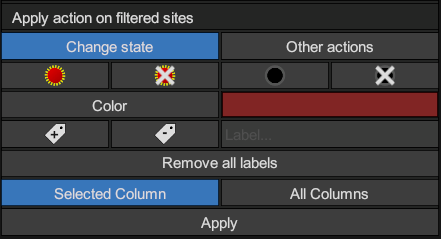
\includegraphics[scale=0.5]{SitesAction.png}
\end{center}
\caption{\label{sitesAction}"Apply action on filtered sites" submenu}
\end{figure}
\paragraph{} The following sections will explain the different functionalities of each toolbar.
\subsubsection{Scene settings}
\begin{figure}[H]
\begin{center}

\includegraphics[scale=0.5]{SceneSettings.png}
\end{center}
\end{figure}
\begin{itemize}
\item Display both parts, only the left part or only the right part of the selected mesh (only works for left-right meshes).
\item Display the edges of the mesh.
\item Switch between the soft cut mode (keep everything behind a cut) and the hard cut mode (cut everything in front of a cut).
\item Make the brain transparent (adjust the transparency using the slider). You can not display the edges when the brain is transparent.
\item Change the colormap of the iEEG values.
\item Change the color of the brain.
\item Change the color of the cuts.
\item Change the threshold of the MRI values (contrast). Use the sliders to change these values.
\item Change the mesh (MNI meshes are available no matter the number of patients, the patient meshes are only available if the patient is alone in the visualization).
\item Change the MRI (patient MRIs are only available if the patient is alone in the visualization).
\item Change the implantation (an implantation is available only if each patient of the visualization has an implantation with the same name)
\end{itemize}
\subsubsection{Display settings}
\begin{figure}[H]
\begin{center}

\includegraphics[scale=0.5]{DisplaySettings.png}
\end{center}
\end{figure}
\begin{itemize}
\item Add or remove a view (maximum 5 views).
\item Set up standard views (3 views with 3 different points of view).
\item Reset the camera position of the selected view.
\item Reset the size of the views (if resized using the handlers).
\item Automatic rotation of the brain (you can set the rotation speed with the slider).
\item Change the camera behaviour (T = trackball camera, O = orbital camera).
\item Take a raw screenshot of the scene which will be saved in the default export directory (set in user preferences).
\item Save the scene as files in a directory named after the name of the visualization in the default export directory (one image per opened view, one image per cut, one image and one svg for the graph, one image for the trial matrices, one csv for each curve containing the values).
\end{itemize}
\subsubsection{Activity settings}
\paragraph{} This toolbar changes depending on the selected column, whether it is Anatomy, iEEG, CCEP or fMRI.
\paragraph{} Common parameters:
\begin{figure}[H]
\begin{center}

\includegraphics[scale=0.5]{ActivitySettings.png}
\end{center}
\end{figure}
\begin{itemize}
\item Trigger global mode (any changes will be applied to all columns)
\item Change the transparency of the activity values on the brain surface
\item Project the activity values on the brain surface and volume or clean the brain.
\end{itemize}
\paragraph{} iEEG specific parameters:
\begin{figure}[H]
\begin{center}

\includegraphics[scale=0.5]{iEEGSettings.png}
\end{center}
\end{figure}
\begin{itemize}
\item Change the size of the influence sphere of the sites (to compute the iEEG on the brain surface)
\item Change the threshold values for the iEEG (anything less than the minimum value will be of the same color as the minimum value, the same apply for the maximum value; the rest of the values will increase linearly from minimum to middle and then increase linearly from middle to maximum). You can change these values by either using the sliders or editing the numbers in the boxes. There are 2 modes : the symmetric mode allows you to set the middle value and the amplitude, whereas the asymmetric mode allows you to set each value independently.
\item Compute and display the correlations between all sites in a single patient visualization. See Appendix \ref{correlations} for more information about the computation method. You can also save and load correlations files.
\end{itemize}
\paragraph{} CCEP specific parameters:
\begin{figure}[H]
\begin{center}

\includegraphics[scale=0.5]{CCEPSettings.png}
\end{center}
\end{figure}
\begin{itemize}
\item Toggle between single site source or MarsAtlas area source
\item Set or unset the selected site as source
\item Select the MarsAtlas area to be used as source
\item Change the size of the influence sphere of the sites
\item Change the threshold values
\end{itemize}
\paragraph{} fMRI specific parameters:
\begin{figure}[H]
\begin{center}

\includegraphics[scale=0.5]{fMRISettings.png}
\end{center}
\end{figure}
\begin{itemize}
\item Change the threshold values of the fMRI. Unlike the iEEG and CCEP threshold values, there are 4 threshold values: all values under the maximum negative slider will be of the same color; all values between the minimum negative and minimum positive sliders will be of the same color; all values above the maximum positive slider will be of the same color; any value between the two negative sliders or the two positive sliders will decrease or increase linearly.
\item Hide the values that are not between the two negative sliders or the two positive sliders
\end{itemize}
\subsubsection{Timeline}
\begin{figure}[H]
\begin{center}

\includegraphics[scale=0.3]{Timeline.png}
\end{center}
\end{figure}
\begin{itemize}
\item Trigger global mode (any changes will be applied to all columns).
\item Make the timeline play automatically.
\item Increase the current timeline ID by a specific amount of samples (this also controls the speed of the play, X samples will be played each second).
\item Loop the timeline (when playing automatically).
\item Slider to control the timeline precisely; the red mark indicates the main event, the blue marks indicates the secondary events (as defined in the protocol).
\item Record a .avi video of the timeline (does not work for fMRI columns)
\end{itemize}
\subsubsection{Sites}
\begin{figure}[H]
\begin{center}

\includegraphics[scale=0.5]{Sites.png}
\end{center}
\end{figure}
\begin{itemize}
\item Selected site name.
\item Display all sites in the scene.
\item Hide blacklisted sites.
\item Change the size of the sites.
\item Compare two sites : select a site, click on this button, then select another site to compare them.
\item Load the single patient scene corresponding to the patient whose site is selected.
\item Cut the brain mesh around the select site. While this setting is on, the cut will be applied each time a site is selected.
\item Move all sites to a selected hemisphere using a symmetry plane. This will only move them visually and it does not affect any computation process.
\item Copy the states of the sites of the selected column to every other columns.
\item Save the states of the sites in a .csv file.
\item Load a .csv file with the states of the sites to the selected column.
\item Open the HBP Interactive Viewer centered around the selected site.
\end{itemize}
\subsubsection{Regions of Interest}\label{roi}
\paragraph{} Regions of Interest (ROI) are useful if you only want to study a small group of sites. They are composed of multiple spheres with different positions and radiuses. If the option "Show All Sites" of the sites toolbar is not enabled, only the sites of the selected ROI will be included in the iEEG computations on the brain. A curve will also be generated for the selected ROI of each column (section \ref{graphs}).
\begin{figure}[H]
\begin{center}
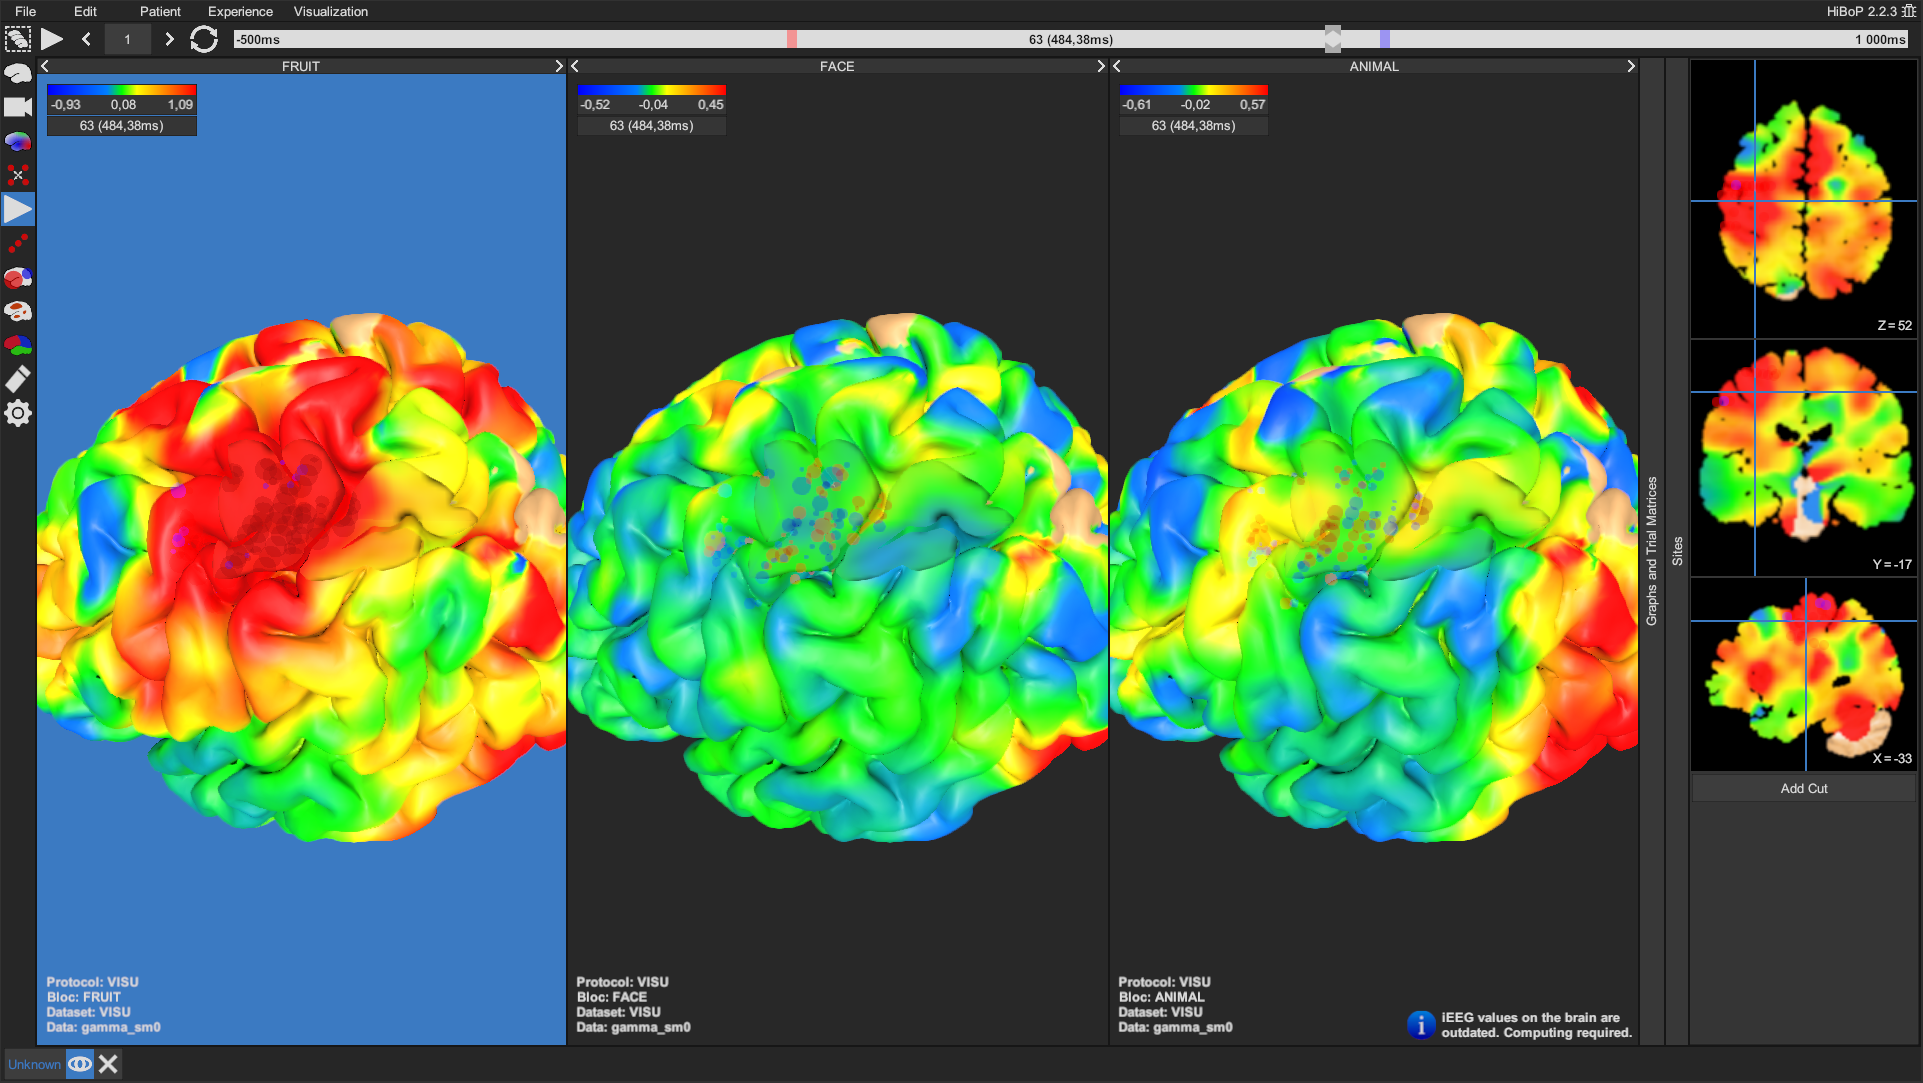
\includegraphics[scale=0.5]{ROI.png}
\end{center}
\end{figure}
\begin{itemize}
\item Add a new ROI in the selected column.
\item Select a ROI for the selected column.
\item Change the name of the selected ROI.
\item Remove the selected ROI.
\item Select a sphere of the ROI.
\item Delete the selected ROI.
\item Copy the selected ROI to other columns.
\item Save the selected ROI to a .roi file.
\item Load a .roi file to the selected column.
\end{itemize}
\paragraph{} After adding a ROI to the selected column, you can left click on the mesh to add spheres to this ROI. You can select a sphere using either the toolbar or by left clicking on it. You can change the position of the selected sphere by draging and droping it and its size using the scroll wheel.
\subsubsection{Atlas}
\begin{figure}[H]
\begin{center}

\includegraphics[scale=0.5]{Atlas.png}
\end{center}
\end{figure}
\begin{itemize}
\item Toggle between MarsAtlas, JuBrain Cytoarchitectonic Atlas, IBC Functional Atlas, and DiFuMo.
\item For MarsAltas and the JuBrain Cytoarchitectonic Atlas, you can visualize the different areas on the 3D brain and hover them to get more information.
\item For the IBC Functional Atlas, you can select the contrast you want to visualize and change the thresholds values.
\item For the DiFuMo atlas, you can select the precision and the area you want to visualize.
\end{itemize}
\subsubsection{Triangle eraser}
\begin{figure}[H]
\begin{center}

\includegraphics[scale=0.5]{TriEraser.png}
\end{center}
\end{figure}
\begin{itemize}
\item Reset the triangle eraser.
\item Choose how you want to erase triangles (one triangle, cylinder, zone). To erase triangles, left click on the mesh where you want to erase them.
\item Expand the erased zone.
\item Invert the erased zone.
\item Revert last action.
\item Save the state of each triangle (invisible or visible) to a .trimask file.
\item Load a .trimask file to apply the states to the triangles of the displayed brain mesh.
\end{itemize}
\subsubsection{Configuration}
\begin{figure}[H]
\begin{center}

\includegraphics[scale=0.5]{Configuration.png}
\end{center}
\end{figure}
\paragraph{} This toolbar allow you to save, load or reset the configuration of the selected scene. Beware, saving the configuration will just save it to the loaded visualization: to write the changes in the corresponding file, you still have to save the whole project. It also allows you to copy the currently selected visualization to a new one saved within the project.
\subsection{Graphs and Trial Matrices}\label{graphs}
\paragraph{} The middle panel allows you to examine more precise information about the iEEG data of specific sites. You can open it using the handlers or if it is closed, it will automatically open once you select a site.
\subsubsection{Graphs}
\begin{figure}[H]
\begin{center}
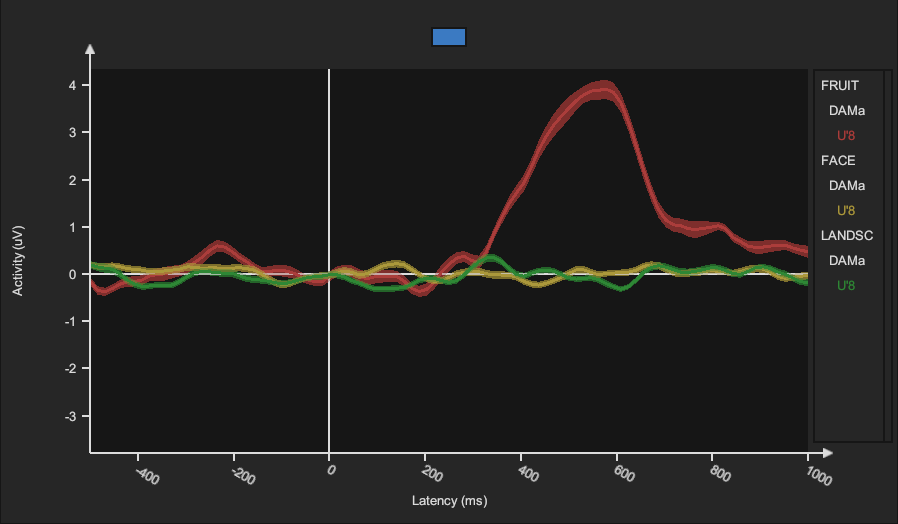
\includegraphics[scale=0.35]{Graph.png}
\end{center}
\caption{\label{graph}Graph for a protocol and three blocs (site U'8)}
\end{figure}
\paragraph{} Curves are generated for each column (or not minimized columns, depending on the chosen preferences):
\begin{itemize}
\item One curve for the last selected site (the column in which the site has been selected does not matter)
\item One curve for the compared site if you are comparing two sites using the "Compare Site" tool in the site toolbar
\item One curve for the ROI if it exists. The ROI is considered as a single site which has the combined activity of all sites (excluding excluded or blacklisted sites) within it.
\end{itemize}
\paragraph{} An example of graph can be found at Figure \ref{graph}. A curve is the mean or median (depending on global preferences) of the iEEG activity of a site. The shapes around the single site curves correspond to the standard error of the mean (SEM). You can interact with the graph in order to get the most of it :
\begin{itemize}
\item You can hover a point with your mouse to see precise coordinates of this point.
\item You can zoom in and out using the mouse wheel and left click and drag to move the graph.
\item You can left click on an axis to precisely edit the viewport of the curve. This small window also has an "Auto" button; this functionality adapts the viewport so you can see every points of each curve.
\item You can hide a curve by left clicking on the corresponding item in the legend.
\end{itemize}
\subsubsection{Trial matrices}
\begin{figure}[H]
\begin{center}
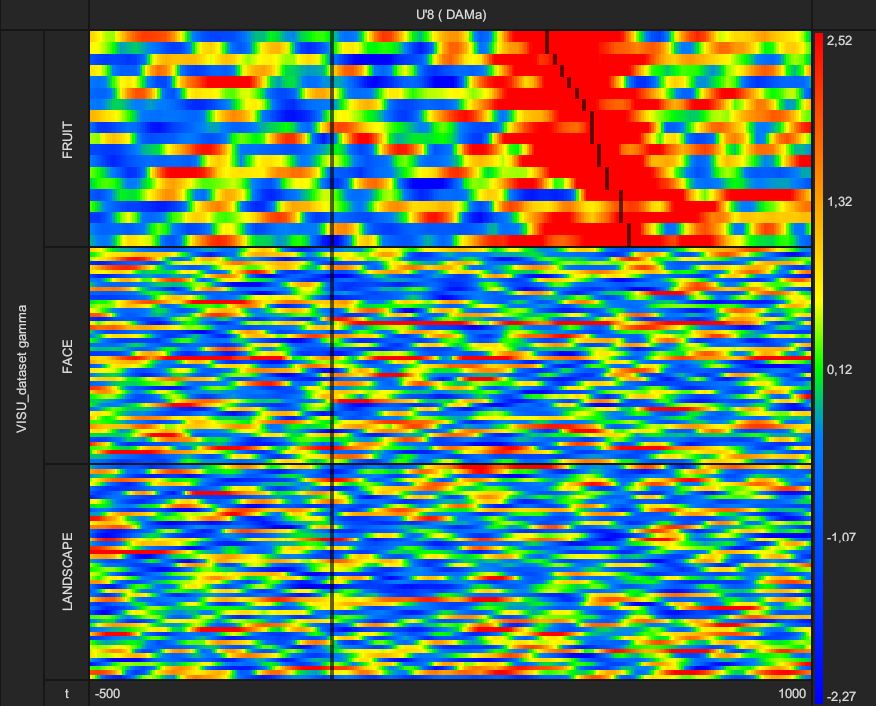
\includegraphics[scale=0.35]{TrialMatrix.png}
\end{center}
\caption{\label{trialMatrix}Trial matrix of a site}
\end{figure}
\paragraph{} Trial matrices are usefull to inspect iEEG activity of a site trial by trial. Trials are sorted according to the sorting method of a protocol bloc. You can change the color scale by clicking on it (same process as changing the viewport of the graph). Again, you can hover the matrix to get precise information about the hovered section (like in graphs). You can also select specific trials; only the selected trials will be taken into account when computing the values of the corresponding curve. To select trials, you can :
\begin{itemize}
\item Select a single trial by left clicking on it
\item Select multiple trials by either shift/ctrl left clicking on the trials you want to select, or by pressing the left click button dragging the mouse and releasing the button.
\item Move the selection with the scroll wheel
\end{itemize}
\subsubsection{Graphs grid}
\begin{figure}[H]
\begin{center}
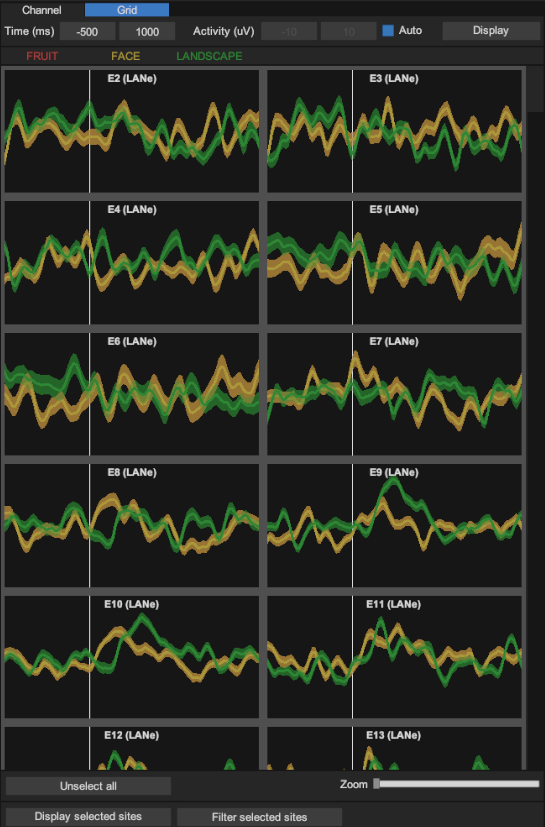
\includegraphics[scale=0.45]{Grid.png}
\end{center}
\caption{\label{graphsGrid}Example graphs grid}
\end{figure}
\paragraph{} The graphs grid can be used to visualize graphs of multiple sites at once. A graph will be generated for each site that is filtered. You can then drag and drop the graph of a site in order to sort them "by hand", select and display or filter them, and change the zoom to visualize more graphs at once.
\appendix
\section{Adding and removing data of a HiBoP project}\label{addobjects}
\subsection{General rule}
\paragraph{} Adding data to a HiBoP project is done using the "+" button to the left of a list containing data objects. Clicking this button will ask you how you want to add data to the project:
\begin{itemize}
\item \textbf{From scratch}: this is the default behaviour when other options are not available. This will create a new object for the given data type that will be completely empty. You will then have to fill the different fields using the object modifier that pops up and save it to add it to the project.
\item \textbf{From existing object}: this option allows you to select an already existing object of the project for the given data type. It will then clone this object to a new object. This can increase the efficiency when creating different objects that have common fields.
\item \textbf{From file}: this allows you to select a file that contains information about an object of a specific data type. The description of the files for every data types is available at section \ref{data}.
\item \textbf{From database}: this allows you to add multiple objects at once using the path to a database. Selecting this option will ask you to browse to a database formatted for the data type you are adding. Once the database is loaded, you can select which objects you want to add and press "OK" to add them all to the project.
\end{itemize}
\paragraph{} Removing data is done by selecting the elements to be removed in the list and using the "-" button to the left of the list.
\subsection{Specific cases}
\subsubsection{Patients}
\paragraph{} Patients are commonly added using a database, because otherwise it is a lot of work adding all the anatomical data one file at a time for all patients of a project. The supported format for the database is the Brain Imaging Data Structure (BIDS) format\footnote{More information about BIDS can be found at http://bids.neuroimaging.io/}. Thus when selecting "From database", you have to browse to a database that is BIDS-compatible.
\subsubsection{Sites}
\paragraph{} While it is possible to select "From file" to add sites to a patient, there is no specific file described in section \ref{data} that concerns sites directly. However, you can still use this option to add multiple sites at once using a specific file format:
\begin{itemize}
\item \textbf{IntrAnat PTS}: this *.pts file contains information about sites positions. It is defined by the IntrAnat format specification.
\item \textbf{IntrAnat CSV}: this *.csv file which separator is tabulation also comes from IntrAnat and is used to get tags for the sites (the name of the tag being in the header of the csv).
\item \textbf{BIDS TSV}: this *\_electrodes.tsv file specified in the BIDS format can be used to add positions and tags at once.
\end{itemize}
\section{Channel correlations}\label{correlations}
\paragraph{} This section explains how the correlations between channels are computed. This is the only statistical computation that is present within HiBoP.
\paragraph{} Let $(A,B)$ be a pair of channels we want to compute correlations of. Let $S_A(i)$ (respectively $S_B(i)$) be the values of the signal of the channel A (respectively B) for the trial number $i$. We compute $R_{ij} = pearson(S_A(i),S_B(j))$ for each pair $(i,j)$ of trials, where $pearson$ represents the computation of the pearson coefficient for the two sets of values. We sort these values into two sets: one set $E_1$ is composed of all the $R_{ii}$, the other $E_2$ is composed of all the $R_{ij}$ where $i \neq j$.
\paragraph{} Then we compute a Wilcoxon rank-sum test between $E_1$ and $E_2$. This gives us a p-value $p$. This p-value is then compared to the "Alpha threshold" value set in the User Preferences of HiBoP, eventually modified using the Bonferroni correction where appropriate.
\paragraph{} More information about this algorithm can be found at https://www.jneurosci.org/content/32/19/6421.
\end{document}